\documentclass{ieeeaccess}
\usepackage{cite}
\usepackage{amsmath,amssymb,amsfonts}
\usepackage{algorithmic}
\usepackage{graphicx}
\usepackage{subcaption}
\usepackage{textcomp}
\usepackage{array}

\usepackage{bm}
\makeatletter
\AtBeginDocument{\DeclareMathVersion{bold}
\SetSymbolFont{operators}{bold}{T1}{times}{b}{n}
\SetSymbolFont{NewLetters}{bold}{T1}{times}{b}{it}
\SetMathAlphabet{\mathrm}{bold}{T1}{times}{b}{n}
\SetMathAlphabet{\mathit}{bold}{T1}{times}{b}{it}
\SetMathAlphabet{\mathbf}{bold}{T1}{times}{b}{n}
\SetMathAlphabet{\mathtt}{bold}{OT1}{pcr}{b}{n}
\SetSymbolFont{symbols}{bold}{OMS}{cmsy}{b}{n}
\renewcommand\boldmath{\@nomath\boldmath\mathversion{bold}}}
\makeatother

\def\BibTeX{{\rm B\kern-.05em{\sc i\kern-.025em b}\kern-.08em
    T\kern-.1667em\lower.7ex\hbox{E}\kern-.125emX}}

%Your document starts from here ___________________________________________________
\begin{document}
\history{Date of publication xxxx 00, 0000, date of current version xxxx 00, 0000.}
\doi{10.1109/ACCESS.2024.0429000}

\title{Multi-Sensor Integration Strategies for Landmine Detection: Data, Feature, and Decision Fusion}
\author{
\uppercase{Ajla Kulaglic}\authorrefmark{1}, \IEEEmembership{Member, IEEE},
\uppercase{Mohammed Baydoun}\authorrefmark{2}, 
\uppercase{Mohammed Al-Husseini}\authorrefmark{1}, \IEEEmembership{Senior Member, IEEE},
\uppercase{Elias Safatly}\authorrefmark{3},
\uppercase{Ali El-Hajj}\authorrefmark{3},
\uppercase{Hassan Ghaziri}\authorrefmark{2}
}

\address[1]{College of Engineering and Technology, 
American University of the Middle East, Kuwait (e-mail: \{ajla.kulaglic, mohammed.al-husseini\}@aum.edu.kw)}
\address[2]{Makassed University of Beirut, Beirut, Lebanon (e-mail: mohbay@gmail.com, hassan.ghaziri@lebcsr.org)}
\address[3]{Electrical and Computer Engineering Department, American University of Beirut, Beirut, Lebanon (e-mail: elhajj@aub.edu.lb) }

\markboth
{Baydoun \headeretal: Preparation of Papers for IEEE TRANSACTIONS and JOURNALS}
{Baydoun \headeretal: Preparation of Papers for IEEE TRANSACTIONS and JOURNALS}

\corresp{Corresponding author: Ajla Kulaglic (e-mail: ajla.kulaglic@aum.edu.kw).}


\begin{abstract}

\end{abstract}

\begin{keywords}
Landmine detection, meta detector, ground penetrating radar (GPR), classification, fusion.
\end{keywords}

\titlepgskip=-21pt

\maketitle

\section{Introduction}
\label{sec:introduction}
Landmine pollution is a critical and enduring consequence of armed conflicts. Antipersonnel mines are inherently indiscriminate and can kill or injure civilians decades after their emplacement. In 2023 alone, a minimum of 5,757 casualties of landmines and explosive remnants of war (ERW) were recorded globally, with 1,983 people killed and 3,663 injured, while the survival status for an additional 111 casualties was unknown \cite{ICBL-CMC2024}. Civilians accounted for $84\%$ of all recorded casualties, with children making up $37\%$ of civilian casualties. The presence of landmines and ERW has devastating economic, social and psychological effects on affected communities, extending far beyond direct casualties. Despite the progress in humanitarian demining efforts, the extent of global contamination is increasing due to ongoing conflicts, the protracted process of landmine clearance, and the inadequacy of financial resources allocated to demining operations. These challenges underscore the importance of advancing detection technologies that can support faster and safer clearance operations. Accordingly, in this study we develop a machine learning model that fuses multiple data modalities to detect and classify landmines. 
The manual use of metal detectors (MDs) remains the first choice in landmine and ERW clearance. Ground penetrating radars (GPRs) are also increasingly employed for detecting newer landmines that have minimal or no metal components. MDs suffer from high false alarm (FA) rates because they struggle to differentiate between the metal in a landmine and harmless metal clutter, making the demining process slow and expensive \cite{Evans2024}. This limitation is exacerbated by newer landmine designs that contain fewer and smaller metal components. In contrast, GPRs are valuable for detecting low-metal or non-metal landmines by identifying abnormalities in soil structure based on electromagnetic characteristics. However, GPRs have their own challenges, as their effectiveness is sensitive to environmental factors such as soil type, temperature, and moisture content, which can lead to high error rates and make GPR-based demining less common than MDs \cite{Evans2024}. Furthermore, GPRs can detect anomalies but often cannot inherently classify them as landmines or determine their type without additional analysis.
Research in landmine detection has evolved from improving conventional MD outputs to leveraging GPR and ML methods, aiming to reduce false alarm (FA) rates and improve detection accuracy. Earlier works focused on enhancing MD-based detection by transforming MD‑audio signals into visual forms for easier interpretation \cite{Kaneko2014}, applying buried-object feature‑extraction and classification techniques \cite{Kruuger2008}, and combining signal detection theory with pattern‑matching algorithms \cite{Collins2000, Tran2012}. In a recent field study, metal detector-based sensors have been used \cite{Lekhak2024}. In this study, Lekhak et al. compared airborne and handheld metal detectors, achieving detection rates up to $98.5\%$ for inert landmines and unexploded ordnance detection (UXO). The results showed limitations for small or low-metal-content targets and cluttered terrains. 
Studies of ML-based GPR interpretation techniques highlight the use of artificial neural networks (ANN), support vector machines (SVM), convolutional neural networks (CNNs), and other deep learning (DL) techniques \cite{Pinar2015}. They included autoencoder-based classification framework \cite{Picetti2018}, application of Faster R-CNN and R-CNN detection models on B-scan GPR images \cite{Pham2018, Kafedziski2018}, hybrid algorithms such as genetic-algorithm designed neural networks for multiobjective optimization \cite{Harkat2019}, improved CNN models for buried-objected detection \cite{Xiang2019} and 3D CNN architectures achieving classification accuracies up to $97\%$. Kalaichelvi \textit{et al}. \cite{Kalaichelvi2025} utilized the AlexNet architecture on synthetic GPR data to classify metallic and plastic objects achieving accuracy of $94.6\%$. 
Further research has introduced convolutional SVM-based networks working on simulated GPR data \cite{Ozkaya2020}, Bi-LSTM models for sequence/image interpretation of GPR B-scans \cite{Ozkaya2021}, generation of synthetic GPR datasets to mitigate data scarcity issues \cite{Warren2021}, and convolutional autoencoder-based clutter-removal methods \cite{Temlioglu2021}.  Additional studies include ML classification using simple statistical features (e.g., mean and standard deviation of GPR images) with near $90\%$ accuracy \cite{Smitha2020}. Recognizing that GPR performance strongly depends on soil dielectric properties, target materials, and antenna characteristics, several researches have analyzed the benefits of circular antenna polarization over linear polarization for richer GPR signal content \cite{Takach2016}, along with methods to extract complex relative permittivity and permeability of materials via guided and unguided electromagnetic waves \cite{Shwaykani2018}, and novel approaches to calculate dielectric constants for low-loss materials \cite{Shwaykani2020}. 
Taken together, these works reflect a clear transition from classical sensor‑based detection towards integrated multisensor fusion and AI-driven GPR data interpretation, laying a robust foundation for contemporary machine-learning-based landmine detection frameworks.
Other researches focused on fusing data from different sensors, such as GPR and MD or EMI to enhance the accuracy.  Pinar \textit{et al}. \cite{Pinar2015} simultaneously collect GPR and EMI data using multi-kernel methods for classification. Genc \cite{Genc2019} applied a multi-feature fusion approach on GPR data combining physics-based and image-based features with support vector machines (SVM), showing improved detection rates but lacking integration with MD data, although the exact accuracy was not reported. Khan et al. \cite{Khan2024} proposed a fusion of GPR and metal induction spectroscopy (MIS) combined with ML-based classification across various soil conditions. Their approach achieved accuracy over $98\%$, demonstrating significant performance gains over single-sensor systems.
Modern approaches increasingly employ multisensor designs, for example combining GPR with thermal and optical cameras \cite{Florez-Lozano2020}, using dual-frequency GPR to reduce FA rates \cite{Garcia-Fernandez2021}, or deploying forward‑looking GPR specifically for shallow-buried mines \cite{Pambudi2021}. The emergence of deep learning (DL) has significantly advanced detection capabilities: convolutional neural networks processing GPR B-scan images have reached high classification accuracies \cite{Wang2022}, and hybrid architectures combining DenseUNet with Bi‑ConvLSTM have been proposed to reconstruct dielectric permittivity maps and classify object types \cite{Wang2021}. 
Beyond detection accuracy, robustness in environmental noise has also been studied. Pambudi et al. \cite{Pambudi2020} developed a robust likelihood ratio test for forward-looking GPR, reducing false alarms under model mismatch scenarios. Vivoli et al. \cite{Vivoli2025} introduces HoloMine, a large-scale synthetic dataset using microwave holographic imagining for landmine detection with deep learning models. Although informative, its use of non-standard sensors and simulated data limits applicability to real-field MD-GPR fusion. While GPR and MD contribute significantly to detection performance, fusion of this data using ML offers superior performance in detection, classification and false alarm reduction. The lack of field-based, multi-sensor, public dataset limits the generalizability of current approaches and presents a major space for future research.
The paper is organized as follows:.......


\section{Data Collection}
The dataset consists of MD and GPR measurements performed using an in-house-designed robotic rail installed over a soil container. The rail is 1.5×1.5 m2 in dimensions and has an arm mounted on a transverse bar to hold the MD or the radar. It is equipped with four stepper motors, two of which operate in conjunction to move the bar in one horizontal direction, whereas the third motor moves the arm in the perpendicular horizontal direction. The last motor also moves the arm but in the vertical direction, either up or down, to set the height of the MD or GPR above the soil.
For MD measurements, a CEIA metal detector is used. The software-controlled robotic arm moves the MD over a grid of 11×10 points, and at each point the magnitude of the MD voltage response is recorded. For the GPR case, the grid is 11×7 points, and at each point a 250-ns ultrawideband pulse in the 1.5–6 GHz frequency range is emitted by a Cayenne radar and its reflection is recorded. The pulse has 512 time samples.
Measurements were performed with MD and GPR for 3 cases: landmine present, soil only case, and soil with-cluttered case. These 3 cases lead to a 3-class classification problem. The landmine used is an inert 3D-printed M59, which is cylindrical in shape and has a diameter of 6 cm and a height of 6 cm. Different types of soil are tested, with different humidity content. In terms of clutter, stones are used in addition to different plastic and metal objects.
For the MD case, a total of 264 measurements are performed, including 108 with a landmine present, 108 with only soil, and 48 with clutter objects. In these measurements, the horizontal and vertical locations of the landmine are changed, as well as the type of soil and clutter. These measurements result in an MD dataset that is 264×11×10 in size. An identical number of measurements are conducted with the GPR, with the same composition (108, 108, and 48, respectively), resulting in a dataset that is 264×11×7×512 in size. There is a clear difference between the MD and the GPR in the number of dimensions, since each MD measurement is a 2D matrix of values, whereas for the GPR, it is a 3D matrix.
Since the landmine and clutter objects are not exactly horizontally centered inside the measurement grid, the datasets can be augmented by performing data flipping in 3 horizontal directions. As a result, the datasets used are actually 1056×11×10 for the MD and 1056×11×7×512 for the GPR.


\subsection{Preprocessing and feature extraction}
Before model training, both MD and GPR datasets undergo preprocessing to reduce measurement variability and improve the comparability of signals across different soil types and clutter configurations. For the GPR data, preprocessing is applied along the temporal dimension using standard signal processing operations. During preliminary experiments, some preprocessing approaches introduced a noticeable drift in the recorded traces. Therefore, each time-series data are centered by subtracting its mean amplitude, which is typically in the range of 9000–9500. This simple normalization step reduces baseline fluctuations and improves the stability of input features, thereby enhancing the performance of subsequent classifiers. Since each GPR scan is composed of 512 time samples at each spatial location, the dataset can be viewed as a 512-frame sequence with spatial dimensions of 11×7. Given the relatively low spatial resolution, the frames are upsampled using bilinear interpolation with a factor of two, producing  22 × 14 images that are more suitable for convolutional neural networks. Additionally, temporal downsampling by a factor of \textbf{four} is applied in some experiments to reduce computational load, yielding sequences of 128 frames and resulting in samples of size 128×22×14. To meet the input requirements of deep learning models, all preprocessed GPR samples are standardized to zero mean and unit variance. For the MD modality, the raw measurements already consist of a 2D spatial grid of 11×10 voltage responses. However, a similar normalization is applied to ensure consistent scaling across the augmented dataset.

Feature extraction is required for traditional machine learning approaches and is performed on both modalities. For GPR data, features are derived from both the original scans and their temporal derivative, which is obtained by differencing consecutive time samples and results in 511×11×7 values. From these volumes, histogram-based descriptors are computed to capture the overall distribution of signal amplitudes, while time-domain statistics such as mean, maximum, minimum and standard deviation are calculated along the temporal axis, each producing an 11×7 feature map. The same set of statistical descriptors is also extracted from the MD measurements, using the spatial grid 11×10 to form comparable feature representations. These features, inspired by prior \cite{Safatly2020}  work on metal detector signal analysis, provide a compact yet informative characterization of the signals and support a robust classification of the three target classes (landmine, soil only, and clutter). The datasets are augmented through horizontal flipping in three directions to account for non-centered target placement within the measurement grid, resulting in a total of 1056×11×10 samples for MD and 1056×11×7×512 samples for GPR, which are subsequently used for both preprocessing and feature extraction stages.

The features are noted in Table~\ref{Table03} with the number of extracted features. The features include building a histogram of all data along the $3$ dimensions. In addition, we compute the mean, maximum, minimum and standard deviation images of the data along the time axis resulting in a total of $11\times7$ features in each case.


\begin{table}
\caption{\textbf{Features Extracted from the GPR Scans}}
\label{Table03}
\setlength{\tabcolsep}{3pt}
\begin{center}
\begin{tabular}{|l|c|}
\hline
\textbf{Feature Name}	& \textbf{Num. of Extracted} \\
 & \textbf{Features} \\
\hline \hline
Overall Max	& 1 \\ \hline
Overall Min	& 1 \\ \hline
Overall Standard Deviation	& 1 \\ \hline
Overall Max of Derivative Scan	& 1 \\ \hline
Overall Min of Derivative Scan	& 1 \\ \hline
Overall Standard Deviation of Derivative Scan &1 \\ \hline
Histogram of Scan (8 bins)	& 8 \\ \hline
Histogram of Derivative Scan (8 bins)	& 8 \\ \hline
Mean Image Values	& 11$\times$7 = 77 \\ \hline
Max Image Values	& 77 \\ \hline
Min Image Values	& 77 \\ \hline
Standard Deviation Image Values	& 77 \\ \hline
Derivative Scan Mean Image Values	& 77 \\ \hline
Derivative Scan Max Image Values	& 77 \\ \hline
Derivative Scan Min Image Values	& 77 \\ \hline
Derivative Scan Standard Deviation Image Values	& 77 \\ \hline \hline
\textbf{Total Number of Features}	& \textbf{638} \\
\hline
\end{tabular}
\end{center}
\end{table}

\section{Detection and Classification Methods}
Discriminating landmines from clutter and identifying specific landmine types is formulated as a multi-classification problem. For landmine type identification, each mine or object type is treated as a separate class. The goal is to glassify the object into three main categories: mine, soil, and clutter. 
In this study, several machine learning algorithms were evaluated: logistic regression, bagging, boosting, and convolutional neural networks. 
Logistic Regression (LR) represents a classification algorithm that is used to find a linear relationship between the input features and the probability of the target variable. It uses the logistic function to learn the relationship between the features and target variable by adjusting its parameters to minimize the difference between predicted probabilities and actual outcome. 
Bootstrap aggregating (Bagging) was introduced as an ensemble method designed to improve prediction accuracy by combining the outputs of multiple classifiers. By aggregating the predictions from various models, bagging generally offers better performance than any single classifier. In this study, the random forest (RF) was specifically employed for multiclass classification. Random forest bulbs many trees and makes predictions by averaging the result. 
K-Nearest Neighbors (KNN) represents a non-parametric algorithm that classifies a data point based on the majority label of its nearest neighbors in the dataset. The algorithm calculates its distance from all the other points in the training set. 
Gradient Boosting bulbs a sequence of models where each new model tries to correct the residuals made by the previous models. Each model is trained on the residual errors of the prior model, and the process continues until a stopping criteria is met. 
XGBoost is an optimized version of gradient boosting that is faster and more efficient, with additional features like regularization to prevent overfitting. Like gradient boosting, XGBoost builds a sequence of decision trees, where each tree tries to correct the errors of the previous one. It uses second-order optimization to make the learning process more accurate and efficient. It incorporates regularization to reduce overfitting and improve generalization. 
Convolutional Neural Networks (CNNs) are capable of automatically identifying important features within the data. A CNN consists of  multiple hidden layers, with each layer performing operations such as convolution or pooling. One of the key advantages of CNNs is their translation invariance, meaning they can recognize objects in images regarding their position, which makes them ideal for image classification tasks like the one in this study. 
Since each sample in our dataset can be treated as an image, CNNs are particularly well-suited to handle this type of data. The proposed CNN architecture is divided into two main parts. The first part consists of six convolutional layers, with each pair followed by a max pooling layer and dropout layer. The convolutional layers use a Rectified Linear Unit (ReLU) activation function, and the number of kernels starts at 16 for the first two layers, doubling after each pooling layer. All kernels have a size of 3x3. At the end, we apply a global max pooling layer to extract the features. The second part of the network includes two additional convolutional layers, followed by dropout and global max pooling layer. In contrast to the first part, the convolutional kernels are larger (7x7) and there are a total of 128 kernels. The outputs from both parts of the network are concatenated and passed through two fully connected dense layers with ReLU activation functions with sizes of 128 and 32 neurons, respectively. 

In the following section, we will evaluate the performance of mentioned machine learning models. Additionally, we will explore the significance of feature extraction and the role of ensemble methods in enhancing classification accuracy.


\subsection{Deep Learning Fusion Approach using GPR and MD}
This work aims to combine GPR and MD data which is achieved through a neural-network deep learning model. Deep learning is a subcategory of machine learning that aims to achieve additional insight in the used data by using several layers that utilize non-linear transformations in comparison with a small number of layers. DL networks are considered as the most promising algorithm for ML especially in fields related to imaging. In this work, we utilize both a feature extraction-based approach in addition to a neural network-based approach that uses convolutional layers and recurrent ones to extract the features of the data especially that we are dealing with multi-two-dimensional arrays where each 2D array can be considered as an image. This multi-input or multi-model architecture performs feature-level fusion for classification.
Convolutional neural networks (CNN) are the most used form of image related deep learning and has been proven successful in this field especially that CNNs can automatically extract useful features without using any feature extraction stage as used with other algorithms. The main advantages achieved through CNNs can be attributed to convolutional kernels which find the relations between neighboring information at small scale such as in small neighboring pixels in the form of edges or corners, or larger blocks of images in the form of bigger shapes such as faces, all of which are dependent on the convolutional layer's input. CNNs are generally composed of a set of hidden layers that are mainly either the convolution or pooling operations in addition to others such as batch normalization and dropout.
The GPR and MD data can be handled using several approaches that can combine the data together. Since we need to utilize more than one type, each data type is first normalized as this is a necessary preprocessing step that is also used in previous related works. We initially detail the approach for each data and then the combination method.
First, the GPR data is very similar to video data where each frame can be used as an image and the time axis corresponds to consecutive frames which makes it a candidate for using CNNs or similar architectures. Furthermore, and due to having time dependency, we can use recurrent networks (RNN) that are capable of handling time information and the data changes or updates over time. Therefore, we consider several networks especially when combining convolutional kernels with recurrent ones. Several combinations and layers were attempted at and the best found one is detailed here. It is worth noting that our implementation initially utilized the work in (Zhang, 2018) which implements a set of Pytorch video recognition models.
The used networks’ parameters of the GPR related part are relatively straightforward since these seemed to perform well in our case mainly due to the comparatively small number of samples. The GPR part is composed of two paths. The first path is a standard CNN for a (11, 7, 512) dimensional data and the second path is a standard GRU based RNN for a standard (77, 512) data. Figure~\ref{Fig_GPR} shows the structure of the GPR based NN part. This 2 paths approach is able to provide a more comprehensive set of features.

\begin{figure}
  \centering
  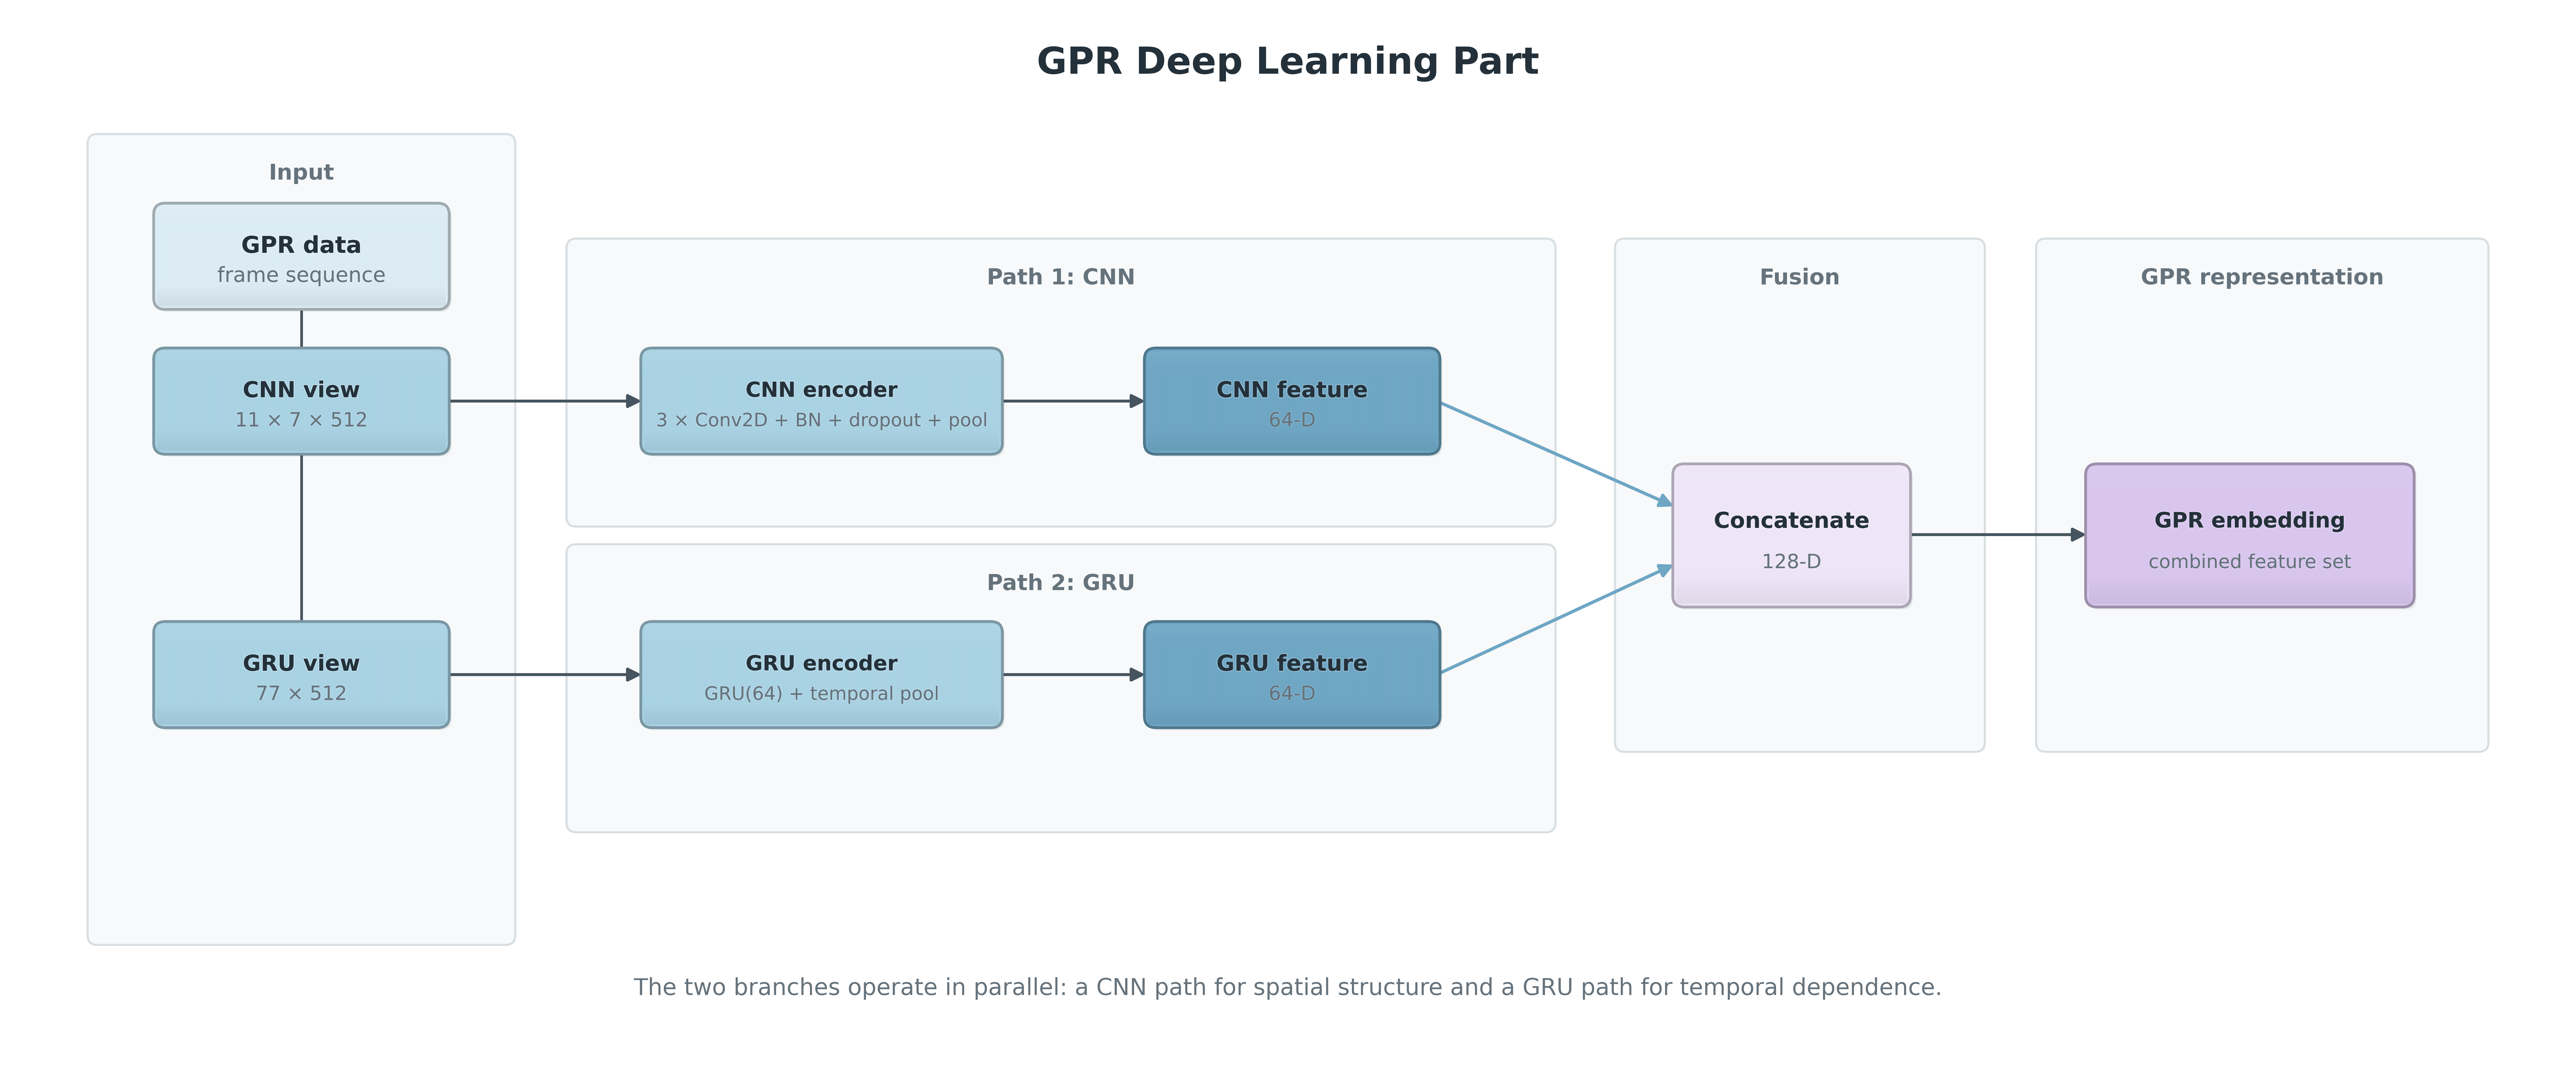
\includegraphics[width=1\linewidth]{./Figures/gpr_deep_learning_part.png}
  \caption{\textbf{GPR Deep Learning Part}}
  \label{Fig_GPR}
\end{figure}


Now, in regards to the MD data, it is similar to a low-resolution grayscale image data, and we utilize a CNN based approach similar to the previous work (Safatly et al). This is a standard convolutional network path as shown in Figure~\ref{Fig_MD}.

\begin{figure}
  \centering
  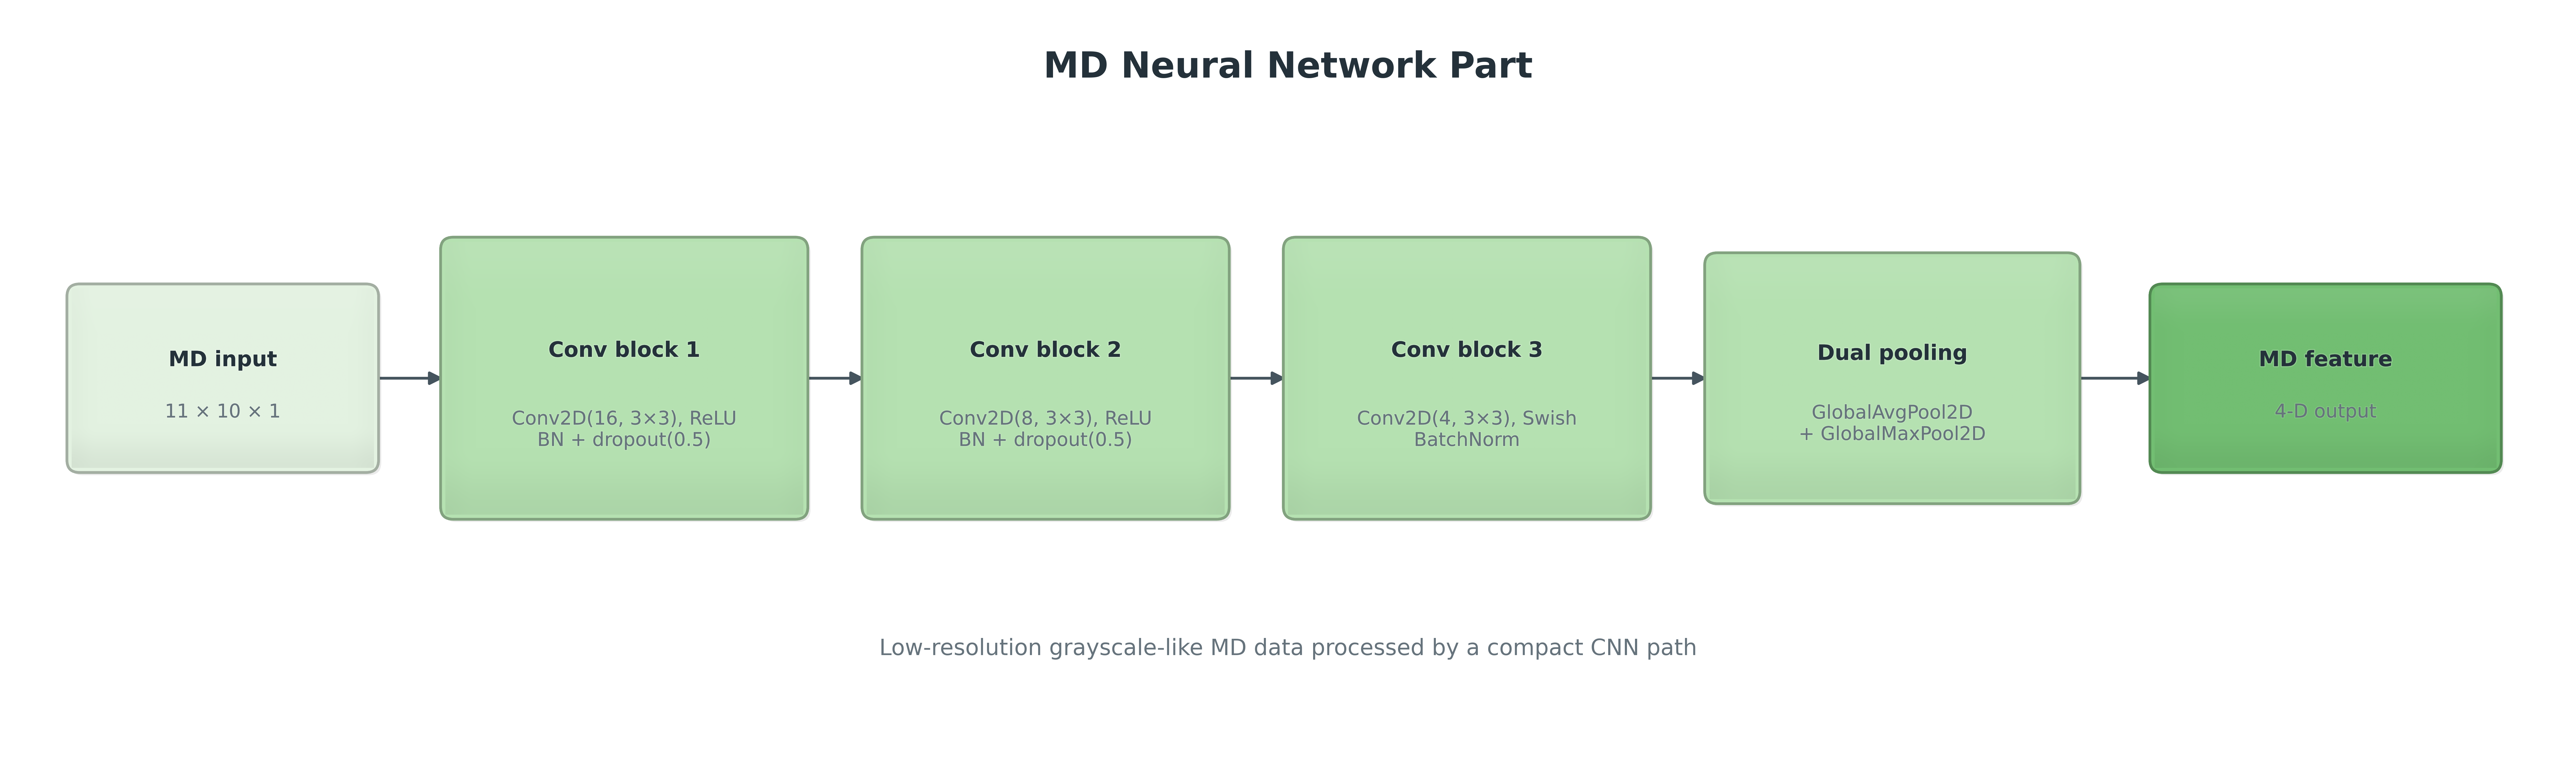
\includegraphics[width=1\linewidth]{./Figures/md_neural_network_part.png}
  \caption{\textbf{MD Neural Network Part}}
  \label{Fig_MD}
\end{figure}

Besides, the extracted statistical features are utilized here since they have proven to benefit accuracy. These have their own standard dense neural network path and are also utilized with the multi-input DL model. Figure~\ref{Fig_Features} shows the basic structure of this part.

\begin{figure}
  \centering
  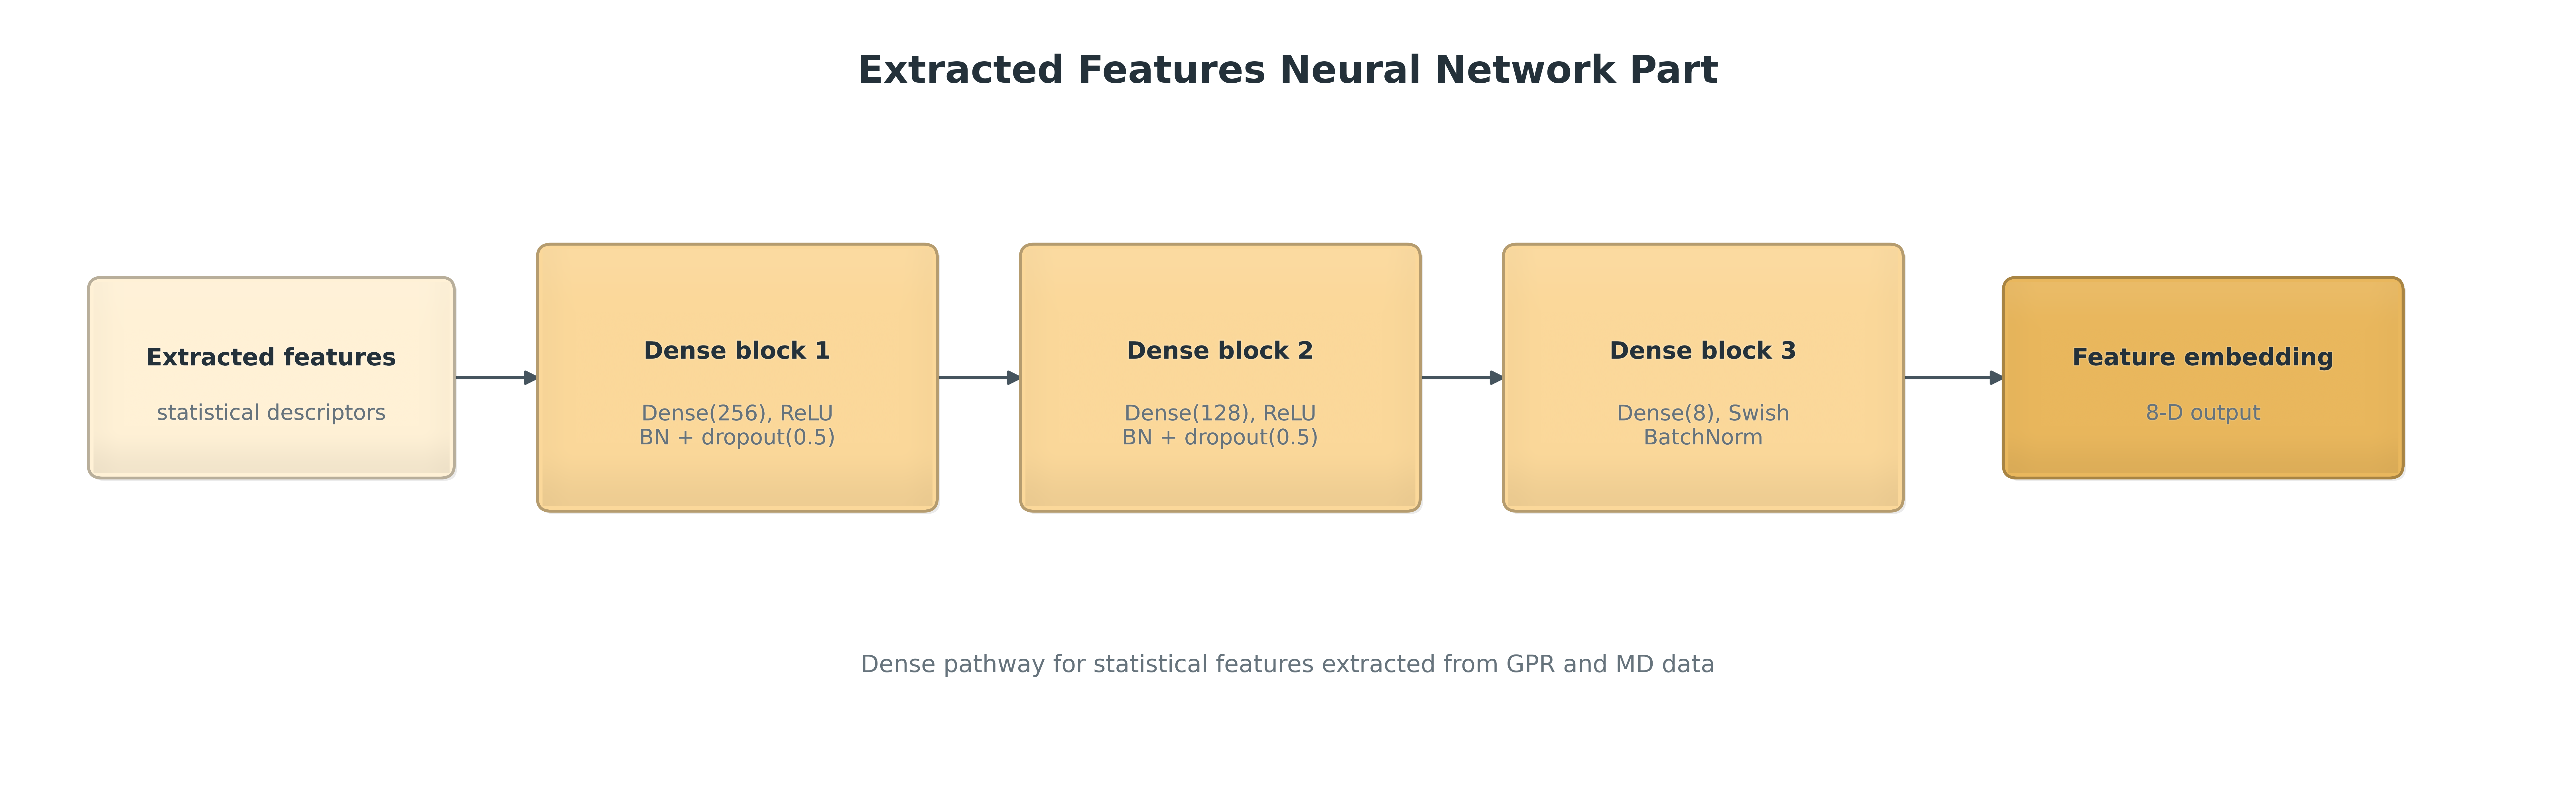
\includegraphics[width=1\linewidth]{./Figures/extracted_features_neural_network_part.png}
  \caption{\textbf{Extracted Features Neural Network Part}}
  \label{Fig_Features}
\end{figure}

 
Each of the different parts are then fused together and we have the final part which is a standard dense neural network path. This multi-input deep learning framework is successful in fusing GPR and metal-detector (MD) data along with the extracted statistical features which are also from both the GPR and MD data. Figure~\ref{Fig_Fusion} shows the combined architecture. It is worth mentioning additional ideas here such as using the Adam optimizer to train the networks with the aid of a learning rate scheduler and utilizing the conventional Rectified Linear Unit (ReLU) as the general activation function. We also use a categorical cross-entropy loss function with Label Smoothing to improve generalization when training the model.

\begin{figure}
  \centering
  \includegraphics[width=1\linewidth]{./Figures/fusion_based_neural_architecture.png}
  \caption{\textbf{Fusion Based Neural Architecture for Combining GPR and MD Landmine Data}}
  \label{Fig_Fusion}
\end{figure}
 



In addition, each data sample or GPR scan can be considered as a video of $512$ frames with a height and width of $11$ and $7$ pixels respectively. Since this video is considered of a low resolution when dealing with convolutional networks, the $11\times7$ matrix can be resized or up-sampled using bilinear interpolation with an up-scaling rate of $2$, so that the size becomes $22\times14$ to be used for deep learning techniques. It is also possible in our case to reduce the sample size along with the size of the time vector through down-sampling by $4$, so that the number of frames becomes $128$ instead of the original $512$. In this case, the data sample size becomes $128\times22\times14$. In addition, deep learning techniques require normalized values. The normalization is standard normalization to produce data to have a mean value of $0$ and a standard deviation of $1$. Other preprocessing methods are possible, but our various tests proved that the selected methods are adequate.



\subsection{Classification}
Determining the buried landmine and distinguishing it from other objects can be addressed as a multi-class classification problem. Identifying the type of the handled problem is a challenge since according to the used data, it is possible to assign a distinct category for each landmine type, each clutter type, each combination of landmine and clutter, and a target free soil. 

As a major discrimination, an important goal is to only consider two categories: mine and non-mine. Three classification problems are therefore considered: the $11$-class problem, the $7$-class problem and the standard binary classification problem with $2$ classes which is the one mainly used in literature. The class labeling of the available samples is used as shown in Table~\ref{Table04}, showing the type of each class either between $1$ to $11$, $1$ to $7$, or $0$ for (no mine) and $1$ for (mine).



\begin{table}
\caption{\textbf{Classes of the Used Objects}}
\label{Table04}
\setlength{\tabcolsep}{3pt}
\begin{center}
\begin{tabular}{|l|c|c|c|}
\hline
\textbf{Object} & \textbf{Class ID} & \textbf{Class ID} & \textbf{Class ID} \\
 & \textbf{(11-class)} & \textbf{(7-class)} & \textbf{(2-class)} \\
 \hline \hline
Mine AP No. 4	& 1	& 1	& 1 \\ \hline
Mine Gyata 64	& 2	& 2	& 1 \\ \hline
Mine M59	& 3	& 3	& 1 \\ \hline
Mine M14	& 4	& 4	& 1 \\ \hline
Mine AP No. 4 with clutter	& 5	& 1	& 1 \\ \hline
Mine Gyata 64 with clutter	& 6	& 2	& 1 \\ \hline
Mine M59 with clutter	& 7	& 3	& 1 \\ \hline
Mine M14 with clutter	& 8	& 4	& 1 \\ \hline
Stone cluster	& 9	& 5	& 0 \\ \hline
Plastic bottle	& 10 & 6 & 0 \\ \hline
Target-free soil	& 11 & 7 & 0 \\
\hline
\end{tabular}
\end{center}
\end{table}


Several classification algorithms are tested to achieve the best possible implementation. Linear Discriminant Analysis (LDA), Support Vector Machines (SVM), Bagging and Boosting are the main machine learning methods applied. Since the data being used is similar to a video feed, several versions of convolutional neural networks are tested. The networks include standard convolutional networks, 3D recurrent convolutional networks and 3D convolutional networks. We next present brief information on the algorithms.

\subsubsection*{Linear Discriminant Analysis}
LDA is a standard classification technique that achieves classification by linearly combining the features based on the data’s means and covariances. It can be used with multi-classification problems which is why it was chosen in this work.

\subsubsection*{Support Vector Machines}
SVM is another common classification algorithm that achieves classification by creating hyperplanes in the feature space to classify data. The hyperplanes of SVM are originally linear but can be converted to nonlinear through the kernel trick or kernelization. Several kernels are possible such as polynomials of varying degrees and radial basis ones. SVM is usually used with binary classification problems but can be extended to multi-classification ones, as in this case. This work initially tests several SVM kernel types such as polynomial and radial based, but the original linear kernel outperforms the other kernel types, thus the related findings are presented here. Several previous works related to landmine detection utilize SVM primarily because it provides a good initial accuracy estimate for feature based binary classification problems.

\subsubsection*{Bagging and Random Forests}
Bagging is a standard ensemble method that combines the outputs from various classification algorithms of the same type to improve the predictions in comparison with the original algorithm. It can be used with single-class, multi-class, and even multi-label problems. Bagging is commonly used with decision trees as its base classifier but it can also be used with other classifiers. It’s worth noting that decision trees are supervised classification algorithms that build a tree-based structure whose nodes utilize the features to differentiate between the different sample classes. These can be of different depths and number of nodes where a single depth or level is often referred to as a decision stump. Decision trees are broadly used as the base classifier for several algorithms such as Bagging and Boosting. Through Bagging, the overfitting of the base classifier is reduced by using a certain number of training sets (T) of similar size through repeated random sampling with replacement from the data. Each of the (T) sets leads to a modified classifier or learner where the output of the Bagging or combined model is obtained through average or weighted voting of the base classifiers.

Bagging focuses on data sampling, but another possible extension is sampling or randomly picking different subsets of features when training each single classifier. This leads to the more general Random Forests which is one of the most widely used tree-based algorithms for classification.

\subsubsection*{Boosting}
Boosting algorithms have proven to deliver the best accuracy with tabular data. These algorithms include AdaboostM1 \cite{Freund1997} for binary classification, AdaBoostM2 \cite{Friedman2001} for multi-class problems, XgBoost \cite{Chen2016}, and LightGBM \cite{Ke2017}. Boosting algorithms are used for binary and multi-classification problems. We test three common and state of the art versions on the extracted features of the GPR data: Adaboost, XgBoost and LightGBM.

Adaboost is one of the first developed methods and is still commonly used in the form of AdaboostM1 for binary classification or AdaboostM2 for multi-class problems. This technique is an ensemble method that requires a number of learners (T), similar to Bagging, where the used learner is a relatively weak learner such as a decision tree of lower depths or a decision stump. The main idea is to assign different weights to the samples to better improve the overall accuracy. This is achieved by initially equating the weights of the samples and updating the weights after every step. This is the general approach for boosting techniques noting that several parameters are possible when combining ideas from Random Forests with Boosting.

In addition, we use the extreme gradient boosting (XgBoost) method proposed in \cite{Chen2016}, and the light gradient boosting machines (LightGBM) proposed in \cite{Ke2017}. These two state of the art methods utilize gradient boosting which relies on predicting the residual errors of previous learners while using the gradient descent algorithm to minimize the required metric and improve the accuracy, as opposed to modifying the sample weights used in Adaboost. XgBoost and LightGBM. This often leads to the most accurate in feature-based classification problems especially that there are several parameters to tune when using these classifiers. These depend on the decision tree or base classifier itself, or on the method to update and combine the different classifiers. A detailed explanation of these algorithms in relation to the mathematical formulation is beyond the scope of this work.

\subsubsection*{Deep Learning Models}
Deep learning is a subcategory of machine learning that aims to achieve additional insight in the used data by using several layers that utilize non-linear transformations in comparison with a small number of layers. DL networks are considered as the most promising algorithm for ML especially in fields related to imaging \cite{Shin2016}. In this work, we utilize convolutional neural networks as a form of deep learning since we are dealing with two-dimensional arrays that can be considered as images.
Convolutional neural networks (CNN) are the most used form of image related deep learning and has been proven successful in this field especially that CNNs can automatically extract useful features without using any feature extraction stage as used with other algorithms. The main advantages achieved through CNNs can be attributed to convolutional kernels which find the relations between neighboring information at small scale such as in small neighboring pixels in the form of edges or corners, or larger blocks of images in the form of bigger shapes such as faces, all of which are dependent on the convolutional layer's input. CNNs are generally composed of a set of hidden layers using either the convolution or pooling operations, where pooling or similar operations are mainly used to resize the images.

The GPR data is very similar to video data where each frame can be used as an image and the time axis corresponds to consecutive frames which makes it a candidate for using CNNs or similar architectures. In addition, given the time dependency, we can use recurrent networks (RNN) that are capable of handling time information and the data updates over time. Therefore, we consider several networks especially when combining convolutional kernels with recurrent ones. We first use a standard CNN with several layers relatively similar to the one used in \cite{Safatly2020}. Another possibility is the 3D-CNN which can be used to process video data with 3D convolutional kernels instead of 2D but requires an additional number of parameters. It is also possible to use a Recurrent Convolutional Network (RCNN) similar to CNN but with an added recurrent layer for the time axis. In addition, this work tests a recurrent 3D-CNN model. In total, 4 types of deep learning models are investigated in this work. Our implementation initially utilized the work in \cite{Zhang2018} which implements a set of Pytorch video recognition models.

The used networks' parameters are relatively simple since simpler models seemed to perform well and generally better in our case due to the relatively small number of samples. We also note that we use the up-sampled preprocessed data as discussed in section 4. The main model for the CNN is composed of three blocks where each block is composed of two convolutional layers followed by a max pooling layer. The first block has $32$ convolutional kernels, the second and third blocks have $64$ and $128$ kernels respectively. Each block is made to have a dropout layer with the dropout ratio set to $0.05$ which helps in avoiding overfitting. After the two blocks, we have a flattening operation followed by two fully connected layers with $256$ units in each. These are then followed by the final softmax layer for classification where the number of units equals to the number of classes. The "Relu" function is used as the activation function in all the convolutional and dense layers.

In regards to the 3D-CNN, we use the same structure for the CNN based model where we replaced the 2D convolutional kernels with 3D ones. Also, for the RCNN model, a recurrent LSTM layer is used, such that it is also followed by the same structure as the CNN. The recurrent layer can be bi-directional noting that the differences between using a bi-directional as opposed to a regular recurrent layer are very minor in this work. It is worth noticing that a reshaping operation is required to allow the use of any recurrent layer such as the "GRU" layer, since they are originally one dimensional that distinguishes the RCNN and R3D models from other models. All the used kernels in the convolutional layers, whether for two- or three-dimensional convolutional operations are set to have a radius equal to $3$ in all directions. In addition, the Adam optimizer is used to train the networks with the default parameters in Tensorflow where the learning rate is $0.001$. Figure~\ref{Fig08} shows an example of the utilized architecture in the case of using RCNN with a GRU recurrent layer without the dropout layers.

\begin{figure*}
\begin{subfigure}{0.48\textwidth}
\centering
  \includegraphics[width=.62\columnwidth]{./Figures/Fig08a.png}
  \subcaption{}
  \label{Fig08a}
\end{subfigure}
\hfill
\begin{subfigure}{.48\textwidth}
  \centering
  \includegraphics[width=.5\columnwidth]{./Figures/Fig08b.png}
  \subcaption{}
  \label{Fig08b}
\end{subfigure}
\caption{\textbf{(a) Complete Architecture for RCNN, (b) General Idea of RCNN Architecture.}}
\label{Fig08}
\end{figure*}

\subsubsection*{Combined Models}
In addition to the various models considered in this work, it is possible to combine some of these models to further improve the results. The combination can be done to two or more models, but it is restricted in this work to two models. Combining models can potentially leverage the advantages of each of the combined models. 

The standard method for combining models is to average or sum the outputs according to predetermined weights. However, in this work we consider a safe approach which mainly accepts the solution that indicates the presence of a mine if there is a conflict between the two classifiers. This considered approach is crucial for the deminer's safety which is the key requirement in the demining domain. This could lead to a high false alarm rate which lowers the overall accuracy. As a result, the false alarm rate of the multi-classifier system is likely to decrease. 

In this paper, we look at two different combinations: the first is combining RCNN and Bagging which is considered to check the effect of combining the best EL and DL models. The second combination is using RCNN and CNN models which are the two top performing single models as later shown. It is important to note that the combined models might disagree about the type of mine, and in such cases the output of the RCNN is preferred since it achieves the highest accuracy.


\section{Results}
This section presents the results of using the different classification algorithms including LDA, SVM, Adaboost, Bagging, Xgboost, LightGBM, the four different CNN models and the two combined models. As done in our previous work \cite{Safatly2020}, we use $3$-fold cross validation to validate the accuracy and performance of the different algorithms. In addition, to validate the results using a standard k-fold technique, we report the results using $10$-folds cross-validation which are generally similar to the $3$-fold results while being slightly less accurate and with higher standard deviation. 

We emphasize that using $3$-folds is more adequate due to the nature of the experiments and collected data since each fold would have an equal number of samples of the same object except for class-$2$ and class-$7$. The $3$-fold scheme ensures that the number of instances of each class in all the folds is similar to help reduce the bias in the results.

In addition, augmentation is used to increase the size of the data for each fold separately to $544$ samples per fold. In each training fold, $2$ folds are used for the training, and the others are for testing, which is repeated $3$ times to obtain the average accuracy over all the folds.

For the purpose of evaluating different algorithms, we first use the accuracy for both the multi-class and the binary classification problems. Also, we calculate the confusion matrix since it is commonly used with multi-class problems. The confusion matrix compares between predicted and true outputs. It is composed of columns and rows where the columns correspond to the required true target and the rows correspond to the predicted output. $100\%$ accuracy can be obtained when all the elements outside the diagonal are 0 since these correspond to errors.
Each of the used algorithms has a different set of parameters suitable for improving the results. This work uses the default parameters in sklearn \cite{Pedregosa2011} algorithms or for other algorithms, which means that there is room for improving the results in the future by better tweaking the parameters especially in cases such as XgBoost and LightGBM. Table~\ref{Table05} presents the accuracy results along with the standard deviation of the tested classification algorithms in the $11-$class case for both $3$-folds and $10$-folds cross validation.

\begin{table}
\caption{\textbf{Percentage Accuracy Results for the $11-$Class Problem}}
\label{Table05}
\setlength{\tabcolsep}{3pt}
\begin{center}
\begin{tabular}{|c|c|c|}
\hline
\textbf{Method}	& \textbf{3-fold Accuracy $\pm$ (std)}	& \textbf{10-fold Accuracy $\pm$ (std)} \\ \hline \hline
LDA	& 94.6 $\pm$ (1.2)	& 94.8 $\pm$ (1.3) \\ \hline
SVM	& 93.4 $\pm$ (2.1)	& 92.2 $\pm$ (2.7) \\ \hline
Bagging	& 93.8 $\pm$ (1.2)	& 93.3 $\pm$ (2.1) \\ \hline
Adaboost	& 88.1 $\pm$ (1.6)	& 86.5 $\pm$ (2.9) \\ \hline
XgBoost	& 89.4 $\pm$ (1.0)	& 88.5 $\pm$ (2.1) \\ \hline
LightGBM	& 89.3 $\pm$ (1.1)	& 89.2 $\pm$ (1.5) \\ \hline
CNN	& 96.6 $\pm$ (0.9)	& 96.3 $\pm$ (1.2) \\ \hline
RCNN	& 98.3 $\pm$ (0.8)	& 97.7 $\pm$ (1.3) \\ \hline
3DCNN	& 95.7 $\pm$ (1.6)	& 95.3 $\pm$ (1.9) \\ \hline
R3D	& 97.2 $\pm$ (1.3)	& 96.2 $\pm$ (1.6) \\ \hline
RCNN  $+$ Bagging	& 98.4 $\pm$ (1.0)	& 98.2 $\pm$ (1.2) \\ \hline
RCNN$+$ CNN	& 99.1 $\pm$ (0.8)	& 98.7 $\pm$ (1.0) \\
\hline
\end{tabular}
\end{center}
\end{table}


Confusion matrices are also computed and presented for some algorithms including the LDA algorithm in Figure~\ref{Fig09}, the Bagging algorithm in Figure~\ref{Fig10}, and the CNN based approach in Figure~\ref{Fig11}. The confusion matrices here are reported for one typical fold to better show the exact integer number of samples and they are thus slightly different from the results of Table~\ref{Table05}. The confusion matrices for the different methods indicate that the errors generally occur between mines, but not between mines and non-mines. Also, these matrices highlight that the accuracy for soil without mines is always near $100\%$. Moreover, Mine M59 followed by Mine M14 generally had the lowest accuracy which may be attributed to having the smallest dimensions indicating that the shape of the buried object is a very important property when using the GPR sensor.


\begin{figure}
  \centering
  \includegraphics[width=1\linewidth]{./Figures/Fig09.png}
  \caption{\textbf{Example Confusion Matrix for LDA.}}
  \label{Fig09}
\end{figure}

\begin{figure}
  \centering
  \includegraphics[width=1\linewidth]{./Figures/Fig10.png}
  \caption{\textbf{Example Confusion Matrix for Bagging.}}
  \label{Fig10}
\end{figure}

\begin{figure}
  \centering
  \includegraphics[width=1\linewidth]{./Figures/Fig11.png}
  \caption{\textbf{Example Confusion Matrix for CNN.}}
  \label{Fig11}
\end{figure}

In addition to the $11-$class problem, it is important to report on the results of the $7-$class problem which generally offers better performance except in the case of LDA. Table~\ref{Table06} presents the relevant accuracies. In these cases the CNN related methods also yield the best performance.


\begin{table}
\caption{\textbf{Percentage Accuracy Results for the $7-$Class Problem}}
\label{Table06}
\setlength{\tabcolsep}{3pt}
\begin{center}
\begin{tabular}{|c|c|c|}
\hline
\textbf{Method}	& \textbf{3-fold Accuracy $\pm$ (std)}	& \textbf{10-fold Accuracy $\pm$ (std)} \\ \hline \hline
LDA	& 94.1 $\pm$ (3.0)	& 96.1 $\pm$ (2.3) \\ \hline
SVM	& 95.8 $\pm$ (1.5)	& 95.8 $\pm$ (1.5) \\ \hline
Bagging	& 95.6 $\pm$ (0.9)	& 94.8 $\pm$ (2.7) \\ \hline
Adaboost	& 92.3 $\pm$ (0.9)	& 89.2 $\pm$ (3.6) \\ \hline
XgBoost	& 95.2 $\pm$ (0.7)	& 94.4 $\pm$ (2.9) \\ \hline
LightGBM	& 93.9 $\pm$ (1.3)	& 93.7 $\pm$ (2.6) \\ \hline
CNN	& 97.3 $\pm$ (1.1)	& 96.5 $\pm$ (1.5) \\ \hline
RCNN	& 99.2 $\pm$ (0.5)	& 98.7 $\pm$ (1.3) \\ \hline
3DCNN	& 96.1 $\pm$ (2.1)	& 95.4 $\pm$ (2.3) \\ \hline
R3D	& 97.5 $\pm$ (1.5)	& 97.5 $\pm$ (1.5) \\ \hline
RCNN  $+$ Bagging	& 99.1 $\pm$ (0.6)	& 98.6 $\pm$ (1.1) \\ \hline
RCNN$+$ CNN	& 99.3 $\pm$ (0.4)	& 98.9 $\pm$ (0.9) \\
\hline
\end{tabular}
\end{center}
\end{table}


Beside the $11-$class and $7-$class problems, the binary classification problem is tested using different algorithms and more than $98\%$ accuracy is obtained in all cases. Table~\ref{Table07} shows the corresponding results.


\begin{table}
\caption{\textbf{Percentage Accuracy Results for the Binary Classification Problem}}
\label{Table07}
\setlength{\tabcolsep}{3pt}
\begin{center}
\begin{tabular}{|c|c|c|}
\hline
\textbf{Method}	& \textbf{3-fold Accuracy $\pm$ (std)}	& \textbf{10-fold Accuracy $\pm$ (std)} \\ \hline \hline
LDA	& 98.3 $\pm$ (0.7)	& 99.2 $\pm$ (1.1) \\ \hline
SVM	& 99.3 $\pm$ (0.0)	& 99.3 $\pm$ (1.1) \\ \hline
Bagging	& 98.1 $\pm$ (1.0)	& 98.1 $\pm$ (2.2) \\ \hline
Adaboost	& 99.2 $\pm$ (0.7)	& 98.5 $\pm$ (1.6) \\ \hline
XgBoost	& 98.9 $\pm$ (1.3)	& 98.5 $\pm$ (1.1) \\ \hline
LightGBM	& 98.2 $\pm$ (1.5)	& 98.5 $\pm$ (1.1) \\ \hline
CNN	& 100 $\pm$ (0.0)	& 100 $\pm$ (0.0) \\ \hline
RCNN	& 100 $\pm$ (0.0)	& 100 $\pm$ (0.0) \\ \hline
3DCNN	& 100 $\pm$ (0.0)	& 100 $\pm$ (0.0) \\ \hline
R3D	& 100 $\pm$ (0.0)	& 100 $\pm$ (0.0) \\ \hline
RCNN  $+$ Bagging	& 99.9 $\pm$ (0.1)	& 99.9 $\pm$ (0.1) \\ \hline
RCNN$+$ CNN	& 100 $\pm$ (0.0)	& 100 $\pm$ (0.0) \\
\hline
\end{tabular}
\end{center}
\end{table}

It is important to note that the errors using binary classification are always on the safe side since no false negatives are found in this case. An example, confusion matrix is presented in Figure~\ref{Fig12} for the output achieved using LDA and having a relatively lower accuracy. It is notable that no mines were missed. This could be attributed due to the imbalance in the data since most measurements are mines and this should be an important challenge to consider in future work where collection of the data should concentrate on the landmines in different configurations.

\begin{figure}
  \centering
  \includegraphics[width=0.75\linewidth]{./Figures/Fig12.png}
  \caption{\textbf{Example Confusion Matrix for LDA.}}
  \label{Fig12}
\end{figure}

Thus, it is easier to distinguish between mines and non-mines as opposed to considering different categories for mine and clutter. This can also be noticed in the confusion matrices for the $11-$class case where errors generally occurred when confusing between mines of different types as opposed to differentiating between mines and non-mines. These results are further discussed in the next section.

\section{Discussion}
The presented work shows the effectiveness of using GPR for landmine detection, as suggested by relevant literature, particularly in the case of low-metal-content mines. Among the tested algorithms, DL models deliver the best scores. The binary classification problem has a $100\%$ accuracy, demonstrating the advantage of using GPR to detect landmines especially without metallic parts. We next discuss data-related issues, the outcomes of machine learning algorithms, computational requirements, and potential directions for future research.

\subsection{Data-Related Discussion}
In this work, we rely on a data acquisition setup that uses the GPR UWB radar. Using other types of sensors would lead to the creation of a new database. In such a case, all data acquisition measurements should be repeated and tested with preprocessing and all the subsequent stages. In order to simplify the data collection process, we use the same setup that was previously used to collect data from metal detectors, but this time with a different sensor.

 The study was restricted to using just one kind of soil. Other types of soil should be employed, and the findings should be validated, as was noted in earlier literature. Therefore, the database must be updated continuously using the data collection process. In addition, this data was collected in a lab environment rather than in the field or outdoors, and this is an issue that should be addressed in the future.

 \subsection{Convolutional Neural Networks and Transfer Learning}
 We discuss ideas regarding the use of CNN architectures, in particular standard networks without complex layers. We also tested other cases including residual networks with several layers, but the results ($>94\%$) were not better than the standard networks chosen in this work, which could be attributed to the relatively small size of the used data.
 
Several modeling architectures were also tested, with the best performing models being indicated in this work. The Keras library \cite{Chollet2018} with a Tensorflow \cite{Abadi2016} backend was mainly used for testing the architectures, in addition, to Pytorch in some cases \cite{Paszke2019}. 

Neural networks require selecting and tuning several parameters, so several ideas were considered in regards to the layers, the activation functions, the kernel sizes, and other parameters. Also, a different number of channels was considered by down-sampling the time-based signals in different ways starting from $512$ to $128$, $64$, $16$ and so on.

We further tested the model using a $3-$channel GPR scan instead of the full or down-sampled model. The three channels were set to the minimum, maximum, and standard deviation. It is therefore possible to directly apply transfer learning to general networks, and the testing resulted in a degradation of performance by about $1\%$ relative to the best obtained results in the case of RCNN. This indicates that it is possible in a future work to consider transfer learning with larger databases using a different number of channels. It is worth noting that this idea of transfer learning has not been used in previous literature on GPR data.

In general, and as shown in Tables \ref{Table05}, \ref{Table06} and \ref{Table07}, CNN based models with augmentation performed the best, especially when combined. Without augmentation, the accuracy decreased, indicating that additional data is required, especially when utilizing CNNs rather than tabular-based classification algorithms like SVM or others.

\subsection{Feature-Related Discussion}
The features employed with the ML models are relatively simple indicating that more features can be added. We tried to use more advanced features such as frequency domain features, peak information features, or advanced signal processing, but the impact on the accuracy was minimal. We also tried the features mentioned in \cite{Abeynayake2019}, but there were no significant improvements. Furthermore, we did not attempt feature selection. The basic extracted features can be considered relevant and have an acceptable corresponding p-value with the output.

\subsection{Combining Models}
Different models were tested for landmine detection and classification. We also combined many models to improve the accuracy as noted in Tables \ref{Table05}, \ref{Table06} and \ref{Table07} for two combined models. It is clear that combining CNN and RCNN leads to the highest accuracy, but this does not rule out the possibility of combining three or more models. and the used scenarios confirm that additional improvement is possible. Furthermore, combining the outputs from the different standard ML models improves the accuracy to more than $98\%$. This indicates that combining models can result in safer and more accurate decisions, especially if the computational time requirements remain acceptable and this would be a very important aspect of any complete system.


\begin{table*}[t]
\caption{\textbf{Comparison with Previous Works}}
\label{Table08}
\setlength{\tabcolsep}{3pt}
\begin{center}
\begin{tabular}{|c|c|c|c|}
\hline
\textbf{Method}	& \textbf{Model(s) Used}	& \textbf{Problem Type}	& \textbf{Accuracy ($\%$)} \\
\hline \hline
\cite{Abeynayake2019} &	SVM/KNN/DT	& Binary	& $97.9$ \\ \hline
\cite{Giovanneschi2019} & SVM and Dictionary Learning	& Multi	& $<80$ \\ \hline
\cite{Moalla2020} &	Deep Learning Models	& Binary	& $<90$ \\ \hline
\cite{Tbarki2021} & Novel version of SVM & Binary with subclasses & $96.8$ \\ \hline
\cite{Wang2022} & 	Deep Learning Models	& Binary	& $94.6$ \\ \hline
\textbf{This work} & Several Machine Learning Models	& Binary/Multi	& Binary: EL$>98$, DL$=100$ \\ 
& & & Multi (7 classes): EL($92-95$), DL($96-99$) \\
& & & Multi (11 classes): EL($89-93$), DL($95-98$) \\
\hline
\end{tabular}
\end{center}
\end{table*}


\subsection{Comparison with Previous Literature}
As already mentioned in the introduction, the authors of \cite{Travassos2020} and \cite{Moalla2020} applied several ML techniques with deep learning methods. Unfortunately, direct comparison with these works is not always practicable due to differences in the data, the experimental setup, and the sensors used. Furthermore, the data from the previous works is not publicly available. However, we discuss the main findings in recent manuscripts to indicate the differences and similarities with our work. 

First, in contrast to earlier work, we investigated additional classes and categories in addition to the standard binary problem, whereas previous literature focused mainly on the binary problem. Although the binary problem is the most important, knowing the type of landmine can help in many cases help with the clearance efforts. Also, understanding the accuracy of the multi-class problem provides additional insight into the classification algorithms' main weaknesses, particularly in cases where a mine is regarded as a clutter, or even a mine with a clutter, indicating that this mine would require extra caution when building the database. Another difference from previous literature is that this work tested several algorithms and found that deep networks outperform standard feature-based classification algorithms when a sufficient amount of data is provided. It is worth highlighting that using data without augmentation affected the performance of deep networks. Furthermore, the sensor utilized in this study is smaller than those used in the literature which makes it suitable for outdoor collection, and this is an advantage because it resulted in similarly accurate results. Table \ref{Table08} summarizes the main differences with previously published directly relevant literature.

Aside from these noted differences, this work agrees with earlier research on several points, such as confirming that more data is required to improve testing and results, whether for a single mine or multiple mines. Despite the differences in the data used, the results obtained are comparable to those obtained in \cite{Abeynayake2019}. Furthermore, it has recently been noted that CNNs can achieve the best performance with GPR data as reported in \cite{Ozkaya2021} and this is validated in this work. Moreover, as shown in \cite{Moalla2020} and \cite{Giovanneschi2019}, adding more sensors or simply making additional measurements with the same sensors can enhance performance. As a result, this work adds to past research and leads to similar conclusions despite using different data and experimental setup.

As an example of comparison with previous literature, we applied the feature extraction stage used in \cite{Abeynayake2019} to our data and performed classification using SVM. In our case, the accuracy results were less than $85\%$ for the binary classification problem, as compared to $97\%$ in the original reference, which is mostly attributed to the differences in the data whether in terms the type of sensors used or even the nature of the data. Abeynayake \textit{et al.} in \cite{Abeynayake2019} used B-scans which are 2D images whereas the data in this work is 3D as previously described. This high discrepancy in accuracy highlights the need for a common database to allow for a more relevant direct comparison with past work, which is the primary motivation for open-sourcing our own database.


\subsection{Notes on Computation Times}
For the ML-based approaches, both feature extraction and predicting the class of the input sample require a small amount of time. The feature extraction process consumes less than $50$ milliseconds on an Intel i7 CPU running at $2.4$ GHz, and the prediction process takes less than $10$ milliseconds when using any of the tested ML models. In comparison, the deep learning models require more time, but still less than $1000$ milliseconds even with recurrent and 3D based models which are known to require more computational time. In all cases, the timing involved is minimal when compared with the data acquisition process which exceeds 5 minutes. This relatively small computational time indicates that combining several models is recommended since time is not a limitation in this case and could be applied to GPR based data or even data from other sensors.


\subsection{Challenges and Future Work}
This research produced encouraging results in terms of landmine detection and classification accuracy using GPR data, but it faced several challenges. As previously stated, collecting the data is the major challenge. This comprises multiple sub-challenges, the first of which is to choose the right GPR sensor, as there are various types of GPR scanners. Another key issue is the mines' availability, or the ability to discover similar objects with almost equal GPR responses. In this work, we chose to use the 3D-printed inert prototypes with parts having similar dielectric constants to the actual materials in the landmines. Another challenge is in the used soil type and its different conditions, which was not addressed in this work that used a single type of soil in similar conditions. Furthermore, obtaining a balanced dataset that accounts for various mine circumstances (orientations, depths, etc.) throughout the data collection phase, as well as during the classification step, where balanced data is preferable, is not a straightforward task. Most of these issues are easier to address when creating a larger field-based database than a lab-based one.

As a result, it is important to define the key requirements for future work:
\begin{itemize}
    \item Obtain more data with different soil types and various soil conditions.
    \item Add other clutter objects to the database.
    \item Combine our previous work in \cite{Safatly2020} that uses a metal detector along with a GPR sensor, which would further improve the accuracy and have added value by targeting both low and high metal content landmines.
    \item More generally as compared to the previous item, mix up the sensor types to produce a comprehensive database from diverse sources.
    \item Perform field testing as it is essential to ensure that the work is fully validated.
\end{itemize}



\section{Data Availability and Access}
We open-sourced the dataset collected for this work and made it publicly available at GitHub through the following link: https://github.com/briclb/GPR.



\section{Conclusion}
GPR lab based data to address the landmine detection is collected.  Several machine learning and deep learning algorithms ranging from standard SVM to boosting techniques to recurrent and convolutional networks are tested to accurately classify landmines and distinguish them from non-mine objects. The obtained results have shown high accuracies in detecting and classifying landmines, especially when combined and achieving a $100\%$ accuracy when addressing the binary classification problem of distinguishing between mines and non-mines on the data. The algorithms can assist the deminer in making accurate decisions about a buried target without having to rely on the GPR's complex graphs or signals. This could result in a faster and more efficient landmine detection and clearance process, with numerous advantages including increased safety and lower total demining costs. More data will expand the database, which we are making public, and is expected to result in a more intelligent detection and classification system especially when field data is collected.




\section*{Acknowledgment}
This work was partially funded by a University Research Board fund from the American University of Beirut (AUB). The authors would further like to thank the Lebanon Mine Action Center (LMAC) and Mr. Stuart Henley for their help.


\bibliographystyle{IEEEtran}
\bibliography{References}

%\newpage

%If you do not have or do not want to include a photo, you can use IEEEbiographynophoto as shown below:


\begin{IEEEbiography}[{
\includegraphics[width=1in,height=1.25in,clip,keepaspectratio]{./Photos/mhusseini_WB.jpg}}] {Mohammed Al-Husseini} (SM'2021) received his Ph.D. in electrical and computer engineering from the American University of Beirut (AUB), Beirut, Lebanon, in 2012. He is currently an assistant professor of computer engineering with the American University of the Middle East (AUM) in Kuwait. Prior to joining AUM, he was a co-founder and research program director with Beirut Research and Innovation Center (BRIC), Beirut, Lebanon, and an electrical and computer engineering lecturer with AUB. Mohammed's research focus is on applied electromagneics, machine learning, and IoT security. He has authored/coauthored 5 book chapters and more than 120 refereed journal and conference papers.
\end{IEEEbiography}


\begin{IEEEbiographynophoto}{Last C. Author, Jr.} (M'87) received the B.S. degree in mechanical
engineering from National Chung Cheng University, Chiayi, Taiwan, in 2004
and the M.S. degree in mechanical engineering from National Tsing Hua
University, Hsinchu, Taiwan, in 2006. He is currently pursuing the Ph.D.
degree in mechanical engineering at Texas A{\&}M University, College
Station, TX, USA.

From 2008 to 2009, he was a Research Assistant with the Institute of
Physics, Academia Sinica, Tapei, Taiwan. His research interest includes the
development of surface processing and biological/medical treatment
techniques using nonthermal atmospheric pressure plasmas, fundamental study
of plasma sources, and fabrication of micro- or nanostructured surfaces.

Mr. Author's awards and honors include the Frew Fellowship (Australian
Academy of Science), the I. I. Rabi Prize (APS), the European Frequency and
Time Forum Award, the Carl Zeiss Research Award, the William F. Meggers
Award and the Adolph Lomb Medal (OSA).
\end{IEEEbiographynophoto}

\EOD

\end{document}
